\chapter{Conjuntos}
\label{cap:conjuntos}

\ifdefined\separatechapter\bookbanner\fi

Asumo que el lector conozca algunas bases de la teoría de conjuntos elemental;
para los que quieran revisarla, recomiendo el libro
\cite{Shen-Vereshchagin-2002}. En este capítulo vamos a recordar ciertas
propiedades de aplicaciones entre conjuntos y además hablar un poco de las así
llamadas ``propiedades universales'', que al principio podrían verse arcanas,
pero van a jugar papel muy importante en nuestro curso. En fin, revisaremos
las relaciones de equivalencia que también tendrán mucha importancia.

\vspace{1em}

Primero recordemos las nociones y notación básica.

\begin{itemize}
\item La cardinalidad de un conjunto $X$ se denota por $|X|$. Normalmente vamos
  a usar esta notación para los conjuntos finitos, es decir cuando $|X|$
  corresponde al número de elementos. Para un conjunto definido por una
  expresión entre llaves $\{ \cdots \}$ a veces se usa la notación
  $\# \{ \cdots \}$, por ejemplo
  $$\# \{ 0,1,2,3 \} = 4.$$

\item Si un elemento $x$ pertenece a un conjunto $X$, se escribe ``$x\in X$'' o
  a veces ``$X \ni x$''.

  \begin{center}
    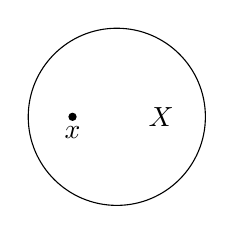
\begin{tikzpicture}[x=0.75cm,y=0.75cm]
      \draw circle (1.5);
      \draw (0.75,0) node {$X$};
      \fill (-0.75,0) circle (1.5pt) node[below] {$x$};
    \end{tikzpicture}
  \end{center}

\item El \term{conjunto vacío} se denota por $\emptyset$. Es el conjunto que no
  tiene ningún elemento:
  $$|\emptyset| = 0.$$

\item Si un conjunto $X$ está contenido en un conjunto $Y$, se escribe
  ``$X\subseteq Y$'' o ``$Y \supseteq X$'':
  $$x\in X \Longrightarrow x\in Y.$$

  \begin{center}
    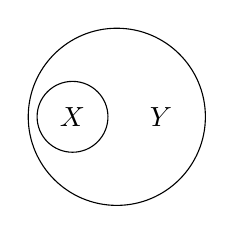
\begin{tikzpicture}[x=0.75cm,y=0.75cm]
      \draw circle (1.5);
      \draw (0.75,0) node {$Y$};
      \draw (-0.75,0) circle [radius=0.6] node {$X$};
    \end{tikzpicture}
  \end{center}

  Tenemos $X = Y$ si y solo si $X\subseteq Y$ e $Y\subseteq X$.

  A veces para subrayar que $X$ está contenido en $Y$, pero $X \ne Y$,
  se escribe ``$X\subsetneq Y$'' o ``$Y \supsetneq X$''. En este caso se dice
  que $X$ es un \term{subconjunto propio} de $Y$.

  La notación $X \not\subseteq Y$ significa que $X$ \emph{no} está contenido en
  $Y$; es decir, que existe $x\in X$ tal que $x \notin Y$. No hay que confundir
  ``$\subsetneq$'' con ``$\not\subseteq$''.

\item La \term{intersección} y \term{unión} de dos conjuntos $X$ y $Y$ se
  denotan por ``$X\cap Y$'' e ``$X\cup Y$'' respectivamente:
  \begin{align*}
    X\cap Y & \dfn \{ z \mid z\in X \text{ y } z\in Y \},\\
    X\cup Y & \dfn \{ z \mid z\in X \text{ o } z\in Y \}.
  \end{align*}

  \begin{center}
    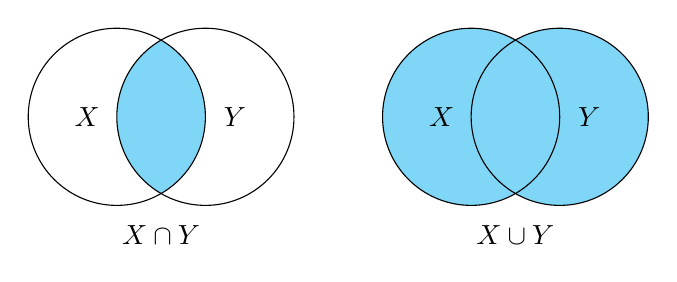
\begin{tikzpicture}[x=0.75cm,y=0.75cm]
      \begin{scope}
        \clip (-0.75,0) circle (1.5);
        \fill[cyan!50] (+0.75,0) circle (1.5);
      \end{scope}

      \draw (-0.75,0) circle (1.5);
      \draw (-1.25,0) node {$X$};
      \draw (+0.75,0) circle (1.5);
      \draw (+1.25,0) node {$Y$};
      \draw (0,-2) node {$X\cap Y$};

      \fill[cyan!50] (+5.25,0) circle (1.5);
      \fill[cyan!50] (+6.75,0) circle (1.5);

      \draw (+5.25,0) circle (1.5);
      \draw (+4.75,0) node {$X$};
      \draw (+6.75,0) circle (1.5);
      \draw (+7.25,0) node {$Y$};
      \draw (+6,-2) node {$X\cup Y$};
    \end{tikzpicture}
\end{center}

De la misma manera, para una familia de conjuntos $X_i$ indexada por $i\in I$
(donde $I$ es algún conjunto, no necesariamente finito), tenemos
\begin{align*}
  \bigcap_{i\in I} X_i & \dfn \{ z \mid z \in X_i \text{ para todo }i\in I \},\\
  \bigcup_{i\in I} X_i & \dfn \{ z \mid z \in X_i \text{ para algún }i\in I \}.
\end{align*}

\item La \term{diferencia} entre dos conjuntos $X$ e $Y$ se denota por
  ``$X\setminus Y$'':
  $$X\setminus Y \dfn \{ x\in X \mid x\notin Y \}.$$

  \begin{center}
    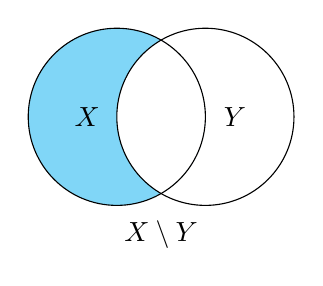
\begin{tikzpicture}[x=0.75cm,y=0.75cm]
      \begin{scope}
        \clip (-0.75,0) circle (1.5);
        \fill[cyan!50,even odd rule] (-0.75,0) circle (1.5) (+0.75,0) circle (1.5);
      \end{scope}

      \draw (-0.75,0) circle (1.5);
      \draw (-1.25,0) node {$X$};
      \draw (+0.75,0) circle (1.5);
      \draw (+1.25,0) node {$Y$};
      \draw (0,-2) node {$X\setminus Y$};
    \end{tikzpicture}
  \end{center}

  Es importante no confundir ``$X \setminus Y$'' con ``$X/Y$'': la segunda
  notación también será usada muy a menudo, pero esta denota un \term{cociente},
  noción que vamos a introducir más adelante.
\end{itemize}

% % % % % % % % % % % % % % % % % % % % % % % % % % % % % %

\section{Aplicaciones entre conjuntos}

Para definir una aplicación $f$ entre un conjunto $X$ y un conjunto $Y$, vamos a
escribir muy seguido
\begin{align*}
  f\colon X & \to Y,\\
  x & \mapsto f (x).
\end{align*}
Note la diferencia entre la flecha ``$\to$'' y ``$\mapsto$''.

\begin{definicion}
  Para una aplicación $f\colon X\to Y$ y un subconjunto $Z \subseteq X$,
  la \term{restricción} de $f$ a $Z$ es la aplicación
  $\left.f\right|_Z\colon Z\to Y$ definida por $\left.f\right|_Z (z) \dfn f (z)$
  para $z\in Z$.
\end{definicion}

\begin{definicion}
  \label{def:imagen-y-preimagen-de-conjunto}
  Para una aplicación entre conjuntos $f\colon X\to Y$ y subconjuntos
  $A \subseteq X$ e $B \subseteq Y$ la \term{imagen} de $A$ es el subconjunto de
  $Y$ dado por
  $$f (A) \dfn \{ f (a) \mid a \in A \}$$
  y la \term{preimagen} de $B$ es el subconjunto de $X$ dado por
  $$f^{-1} (B) \dfn \{ x \in X \mid f (x) \in B \}.$$
\end{definicion}

Notamos que en el segundo caso, ``$f^{-1}$'' es solamente la notación y no se
trata de una aplicación $f^{-1}$.

\begin{observacionejerc}
  Sea $f\colon X\to Y$ una aplicación.

  \begin{enumerate}
  \item[1a)] Para cualquier subconjunto $B \subseteq Y$ se tiene
    $f (f^{-1} (B)) \subseteq B$.

  \item[1b)] Para cualquier subconjunto $A \subseteq X$ se tiene
    $A \subseteq f^{-1} (f (A))$.

  \item[2a)] Si $A_1 \subseteq A_2 \subseteq X$, entonces
    $f (A_1) \subseteq f (A_2)$.

  \item[2b)] Si $B_1 \subseteq B_2 \subseteq Y$, entonces
    $f^{-1} (B_1) \subseteq f^{-1} (B_2)$. \qedhere
  \end{enumerate}
\end{observacionejerc}

\begin{definicion}
  \label{dfn:composicion-de-aplicaciones}
  Para dos aplicaciones $f\colon X\to Y$ e $g\colon Y\to Z$ la
  composición $g\circ f\colon X\to Y$ es la aplicación definida por
  $$(g\circ f) (x) \dfn g (f (x)).$$
\end{definicion}

Esta información puede representarse mediante un ``diagrama conmutativo'':
$$\begin{tikzcd}
X\ar{dr}[swap]{f}\ar{rr}{g\circ f} & & Z \\
 & Y \ar{ur}[swap]{g}
\end{tikzcd}$$

Aclaramos que, para nosotros, la notación ``$g\circ f$'' significa que
\emph{primero} se aplica $f$ y \emph{luego} $g$. Por esto las expresiones como
``$g\circ f$'' a veces se escriben y se leen de derecha a izquierda.
Si $f,g\colon X\to X$ son aplicaciones entre $X$ y sí mismo, entonces ambas
composiciones $g\circ f$ y $f\circ g$ tienen sentido, pero normalmente
el resultado es diferente.

\begin{ejemplo}
  Consideremos las aplicaciones $f,g\colon \RR\to \RR$ definidas por
  $$f\colon x\mapsto x+1 \quad\text{y}\quad g\colon x\mapsto x^2.$$
  Luego,
  \[ g (f (x)) = x^2 + 2x + 1, \text{ mientras que }f(g (x)) = x^2+1. \qedhere \]
\end{ejemplo}

\begin{ejemplo}
  Sea $\phi\colon \RR^2 \to \RR^2$ la rotación del plano de $90^\circ$ en
  el sentido antihorario y sea $\psi\colon \RR^2 \to \RR^2$ la reflexión
  respecto al eje $x$. Estas son aplicaciones lineales que corresponden a
  las matrices
  \[ A = \begin{pmatrix} 0 & -1 \\ 1 & 0 \end{pmatrix}, \quad
    B = \begin{pmatrix} 1 & 0 \\ 0 & -1 \end{pmatrix}. \]
  Se ve géometricamente que $\psi\circ\phi \ne \phi\circ \psi$.

  \begin{center}
    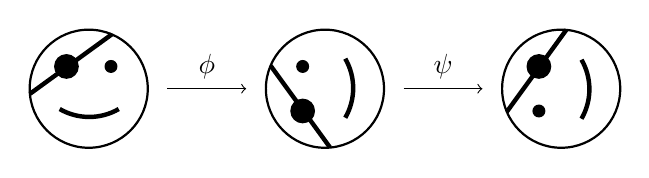
\begin{tikzpicture}[x=0.5cm, y=0.5cm]
      \draw[thick] circle (1.5);
      \draw[fill] (135:0.8) circle (1.5mm);
      \draw[fill] (45:0.8) circle (0.75mm);
      \draw[ultra thick] (185:1.5) -- (67:1.5);
      \draw[ultra thick] (-145:0.9) arc (-120:-60:1.5);

      \begin{scope}[xshift=3cm, rotate=90]
        \draw[thick] circle (1.5);
        \draw[fill] (135:0.8) circle (1.5mm);
        \draw[fill] (45:0.8) circle (0.75mm);
        \draw[ultra thick] (185:1.5) -- (67:1.5);
        \draw[ultra thick] (-145:0.9) arc (-120:-60:1.5);
      \end{scope}

      \begin{scope}[yscale=-1, xshift=6cm, rotate=90]
        \draw[thick] circle (1.5);
        \draw[fill] (135:0.8) circle (1.5mm);
        \draw[fill] (45:0.8) circle (0.75mm);
        \draw[ultra thick] (185:1.5) -- (67:1.5);
        \draw[ultra thick] (-145:0.9) arc (-120:-60:1.5);
      \end{scope}

      \draw [->] (2,0) -- node [above] {$\phi$} (4,0);
      \draw [->] (8,0) -- node [above] {$\psi$} (10,0);
    \end{tikzpicture}

    \vspace{2em}

    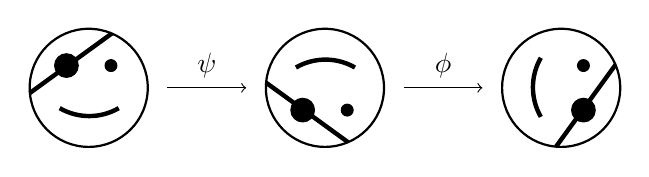
\begin{tikzpicture}[x=0.5cm, y=0.5cm]
      \draw[thick] circle (1.5);
      \draw[fill] (135:0.8) circle (1.5mm);
      \draw[fill] (45:0.8) circle (0.75mm);
      \draw[ultra thick] (185:1.5) -- (67:1.5);
      \draw[ultra thick] (-145:0.9) arc (-120:-60:1.5);

      \begin{scope}[yscale=-1, xshift=3cm]
        \draw[thick] circle (1.5);
        \draw[fill] (135:0.8) circle (1.5mm);
        \draw[fill] (45:0.8) circle (0.75mm);
        \draw[ultra thick] (185:1.5) -- (67:1.5);
        \draw[ultra thick] (-145:0.9) arc (-120:-60:1.5);
      \end{scope}

      \begin{scope}[yscale=-1,xshift=6cm,rotate=-90]
        \draw[thick] circle (1.5);
        \draw[fill] (135:0.8) circle (1.5mm);
        \draw[fill] (45:0.8) circle (0.75mm);
        \draw[ultra thick] (185:1.5) -- (67:1.5);
        \draw[ultra thick] (-145:0.9) arc (-120:-60:1.5);
      \end{scope}

      \draw [->] (2,0) -- node [above] {$\psi$} (4,0);
      \draw [->] (8,0) -- node [above] {$\phi$} (10,0);
    \end{tikzpicture}
  \end{center}

  También podemos multiplicar las matrices:
  \[ BA = \begin{pmatrix} 0 & -1 \\ -1 & 0 \end{pmatrix},
    \text{ mientras que }
    AB = \begin{pmatrix} 0 & 1 \\ 1 & 0 \end{pmatrix}. \qedhere \]
\end{ejemplo}

\begin{observacion}
  \label{obs:composicion-de-aplicaciones-asociativa}
  La composición es \term{asociativa}: para $f\colon X\to Y$,
  $g\colon Y\to Z$, $h\colon Z\to W$ tenemos
  $$(h\circ g)\circ f = h\circ (g\circ f).$$

  \[ \begin{tikzcd}
      X \ar{r}{f}\ar[bend right]{rr}[swap]{g\circ f}\ar[bend left]{rrr}{h\circ g\circ f} & Y \ar{r}{g}\ar[bend right]{rr}[swap]{h\circ g} & Z \ar{r}{h} & W
    \end{tikzcd} \]

  \begin{proof}
    Para cualquier $x\in X$, ambas aplicaciones tienen el valor $h (g (f (x)))$.
  \end{proof}
\end{observacion}

\begin{corolario}[Asociatividad generalizada]
  \label{corr:asociatividad-generalizada-para-composiciones}
  Para $n$ aplicaciones
  $$X_1 \xrightarrow{f_1} X_2 \xrightarrow{f_2} \cdots \to X_{n-1} \xrightarrow{f_{n-1}} X_n \xrightarrow{f_n} X_{n+1}$$
  Toda manera de poner los paréntesis en la expresión
  $$f_n\circ f_{n-1}\circ\cdots\circ f_2\circ f_1$$
  (es decir, de calcular la composición) da el mismo resultado.
\end{corolario}

\begin{ejemplo}
  Para $n = 3$, tenemos dos posibilidades:
  $$(f_3\circ f_2)\circ f_1, \quad f_3\circ (f_2\circ f_1).$$
  El resultado es el mismo según
  \ref{obs:composicion-de-aplicaciones-asociativa}. Para $n = 4$ hay $5$
  posibilidades:
  \begin{gather*}
    ((f_4\circ f_3)\circ f_2)\circ f_1, \quad (f_4\circ (f_3\circ f_2))\circ f_1, \quad (f_4\circ f_3)\circ (f_2\circ f_1), \\
    f_4\circ ((f_3\circ f_2)\circ f_1), \quad f_4\circ (f_3\circ (f_2\circ f_1)). \qedhere
  \end{gather*}
\end{ejemplo}

\begin{comentarioast}
  En general, hay
  $$C_n = \frac{1}{n+1} {2n \choose n} = {2n \choose n} - {2n \choose n+1}$$
  posibilidades de poner los paréntesis en la expresión $f_1\circ\cdots\circ f_n$. Los números $C_n$ se conocen como los \term{números de
    Catalan\footnote{\personality{Eugène Charles
        Catalan}\index{número!de Catalan} (1814--1894), un matemático
      francés-belga.}}.

  \begin{center}
    \begin{tabular}{rx{0.75cm}x{0.75cm}x{0.75cm}x{0.75cm}x{0.75cm}x{0.75cm}x{0.75cm}x{1cm}x{1cm}x{1cm}}
      \hline
      $n\colon$ & $3$ & $4$ & $5$ & $6$ & $7$ & $8$ & $9$ & $10$ & $11$ & $12$ \tabularnewline
      \hline
      $C_n\colon$ & $2$ & $5$ & $14$ & $42$ & $132$ & $429$ & $1430$ & $4862$ & $16796$ & $58786$ \tabularnewline
      \hline
    \end{tabular}
  \end{center}
\end{comentarioast}

\begin{proof}[Demostración de \ref{corr:asociatividad-generalizada-para-composiciones}]
  Para $n = 2$ no hay que demostrar nada y el caso de $n = 3$ es el contenido de
  \ref{obs:composicion-de-aplicaciones-asociativa}. Para $n > 3$, supongamos que
  la propiedad se cumple para toda composición de $< n$ aplicaciones. En una
  expresión $f_n\circ f_{n-1}\circ\cdots\circ f_2\circ f_1$, después de poner
  los paréntesis de algún modo, tenemos
  $$(f_n\circ\cdots\circ f_{r+1})\circ (f_r\circ\cdots\circ f_1),$$
  donde las expresiones en los paréntesis están bien definidas por la hipótesis
  de inducción. Sea
  $$(f_n\circ\cdots\circ f_{s+1})\circ (f_s\circ\cdots\circ f_1)$$
  otro modo de poner los paréntesis. Sin pérdida de generalidad,
  $r < s$. Tenemos
  $$f_n\circ\cdots\circ f_{r+1} = (f_n\circ\cdots\circ f_{s+1})\circ (f_s\circ\cdots\circ f_{r+1})$$
  y
  $$f_s\circ\cdots\circ f_1 = (f_s\circ\cdots\circ f_{r+1})\circ (f_r\circ\cdots\circ f_1).$$
  Ahora
  $$(f_n\circ\cdots\circ f_{r+1})\circ (f_r\circ\cdots\circ f_1) = \bigl((f_n\circ\cdots\circ f_{s+1})\circ (f_s\circ\cdots\circ f_{r+1})\bigr)\circ (f_r\circ\cdots\circ f_1)$$
  y
  $$(f_n\circ\cdots\circ f_{s+1})\circ (f_s\circ\cdots\circ f_1) = (f_n\circ\cdots\circ f_{s+1})\circ \bigl((f_s\circ\cdots\circ f_{r+1})\circ (f_r\circ\cdots\circ f_1)\bigr).$$
  Por inducción, las últimas dos expresiones coinciden.
\end{proof}

Para cualquier conjunto $X$, existe una aplicación distinguida $X\to X$, a saber
la que aplica todo elemento en sí mismo.

\begin{definicion}
  La \term{aplicación identidad}\index{aplicación!identidad}
  $\id{X}\colon X\to X$ se define como\index[notacion]{id@$\idid$}
  $$\id{X} (x) \dfn x.$$
\end{definicion}

\begin{observacion}
  \label{obs:f-circ-id--id-circ-f}
  Para cualesquiera aplicaciones $f\colon X\to Y$ e $g\colon Y\to X$ se cumple
  que
  \begin{equation}
    \label{eqn:f-circ-id--id-circ-f}
    f\circ \id{X} = f, \quad \id{X}\circ g = g.
  \end{equation}
\end{observacion}

Note que \eqnref{eqn:f-circ-id--id-circ-f} define a $\id{X}$ de modo único:
si tenemos dos aplicaciones $i_X', i_X''\colon X\to X$ tales que para
cualesquiera $f\colon X\to Y$ e $g\colon Y\to X$ se cumple
$$f\circ i_X' = f, \quad i_X''\circ g = g,$$
en particular para $X=Y$ tenemos
$$i_X'' = i_X''\circ i_X' = i_X'.$$

\begin{definicion}
  Se dice que una aplicación $f\colon X\to Y$ es \term{invertible}
  \index{aplicación!invertible} si existe otra aplicación
  $f^{-1}\colon Y\to X$ tal que
  \begin{equation}
    \label{eqn:aplicacion-inversa}
    f^{-1}\circ f = \id{X}, \quad f\circ f^{-1} = \id{Y}.
  \end{equation}
\end{definicion}

La notación ``$f^{-1}$'' (no confundirla con la notación de
\ref{def:imagen-y-preimagen-de-conjunto}) está justificada por el hecho de que
la aplicación inversa está definida de modo único.

\begin{observacion}
  Si $f', f''\colon Y\to X$ son dos aplicaciones que satisfacen
  \[ f'\circ f = \id{X}, \quad
    f\circ f' = \id{Y}, \quad
    f''\circ f = \id{X}, \quad
    f\circ f'' = \id{Y}, \]
  entonces $f' = f''$.

  \begin{proof}
    Tenemos
    \[ f' = f'\circ\id{Y} =
      f'\circ (f\circ f'') =
      (f'\circ f)\circ f'' =
      \id{X}\circ f'' = f''. \qedhere \]
  \end{proof}
\end{observacion}

\begin{observacion}
  Si $f\colon X\to Y$ es una aplicación invertible, entonces
  $f^{-1}\colon Y\to X$ es también invertible: su inversa es
  $f\colon X\to Y$:
  $$(f^{-1})^{-1} = f.$$

  \begin{proof}
    Las fórmulas \ref{eqn:aplicacion-inversa} son simétricas y dicen al mismo
    tiempo que $f$ es inversa a $f^{-1}$.
  \end{proof}
\end{observacion}

\begin{observacion}
  \label{obs:aplicaciones-inversas-para-composiciones}
  Si $f\colon X\to Y$ e $g\colon Y \to Z$ poseen aplicaciones inversas
  $f^{-1}\colon Y\to X$ y $g^{-1}\colon Z\to Y$, entonces la composición
  $f^{-1}\circ g^{-1}\colon Z\to X$ es la inversa de $g\circ f\colon X\to Z$.

  \[ \begin{tikzcd}
      X \ar[shift left=.75ex]{r}{f} & Y \ar[shift left=.75ex]{r}{g}\ar[shift left=.75ex]{l}{f^{-1}} & Z\ar[shift left=.75ex]{l}{g^{-1}}
    \end{tikzcd} \]

  En general, toda composición de $n$ aplicaciones invertibles
  $f_n\circ \cdots\circ f_1$ es también invertible y su aplicación inversa es
  dada por
  $$(f_n\circ \cdots\circ f_1)^{-1} = f_1^{-1}\circ\cdots\circ f_n^{-1}.$$

  \begin{proof}
    Tenemos
    \[ (g\circ f)\circ (f^{-1}\circ g^{-1}) =
      g\circ (f\circ f^{-1})\circ g^{-1} =
      g\circ \id{Y}\circ g^{-1} =
      g\circ g^{-1} = \id{Z}, \]
    y de la misma manera,
    \[ (f^{-1}\circ g^{-1})\circ (g\circ f) =
      f^{-1}\circ (g^{-1}\circ g)\circ f =
      f^{-1}\circ \id{Y}\circ f =
      f^{-1}\circ f = \id{X}. \]
    En general, $(f_n\circ \cdots\circ f_1)^{-1}$ se calcula por inducción sobre
    $n$. Acabamos de ver el caso de $n = 2$. Para el paso inductivo, escribamos
    \[ (f_n\circ \cdots\circ f_1)^{-1} =
      (f_n\circ (f_{n-1}\circ\cdots\circ f_1))^{-1} =
      (f_{n-1}\circ\cdots\circ f_1)^{-1}\circ f_n^{-1}. \qedhere \]
  \end{proof}
\end{observacion}

Note que en la fórmula ``$(g\circ f)^{-1} = f^{-1}\circ g^{-1}$'' se cambia
el orden de $f$ y $g$. Es algo natural: la composición $g^{-1}\circ f^{-1}$
no tiene sentido. Piense en el siguiente ejemplo de la vida real: para salir,
primero ponemos una camisa y luego un abrigo. Después, primero se quita
el abrigo y luego la camisa y no al revés.

% % % % % % % % % % % % % % % % % % % % % % % % % % % % % %

\section{Aplicaciones inyectivas, sobreyectivas y biyectivas}
\label{seccion:inyectivas-sobreyectivas-biyectivas}

\begin{definicion}
  \label{dfn:inyectivas-sobreyectivas-biyectivas}
  Una aplicación entre conjuntos $f\colon X\to Y$ es
  \begin{enumerate}
  \item[1)] \term{inyectiva}\index{aplicación!inyectiva} si $f$ aplica
    diferentes elementos de $X$ en diferentes elementos de $Y$; es decir,
    $$f (x) = f (x') \Longrightarrow x=x';$$

  \item[2)] \term{sobreyectiva}\index{aplicación!sobreyectiva} si para todo
    $y\in Y$ existe $x\in X$ tal que $f (x) = y$;

  \item[3)] \term{biyectiva}\index{aplicación!biyectiva} si es inyectiva y
    sobreyectiva al mismo tiempo.
  \end{enumerate}
\end{definicion}

\begin{observacionejerc}
  Sea $f\colon X\to Y$ una aplicación.

  \begin{enumerate}
  \item[1)] Si $f$ es sobreyectiva, entonces para cualquier subconjunto
    $B \subseteq Y$ se tiene ${f (f^{-1} (B)) = B}$.

  \item[2)] Si $f$ es inyectiva, entonces para cualquier subconjunto
    $A \subseteq X$ se tiene ${f^{-1} (f (A)) = A}$. \qedhere
  \end{enumerate}
\end{observacionejerc}

Podemos caracterizar las propiedades de arriba en términos de composiciones de
aplicaciones.

\begin{observacionejerc}
  \label{obs:composicion-de-inyectivas-sobreyectivas-biyectivas}
  Sean $f\colon X\to Y$ e $g\colon Y\to Z$ dos aplicaciones. Si $f$ y $g$ son
  inyectivas (resp. sobreyectivas, biyectivas), entonces $g\circ f$ es también
  inyectiva (resp. sobreyectiva, biyectiva).
\end{observacionejerc}

\begin{proposicion}
  \label{prop:mono-epi-iso-en-Set}
  Sea $f\colon X\to Y$ una aplicación entre conjuntos.

  \begin{enumerate}
  \item[1)] $f$ es inyectiva si y solamente si es cancelable por la izquierda:
    para todo par de aplicaciones $g, g'\colon Z\to X$ tenemos
    \begin{equation}
      \label{eqn:cancelacion-de-mono}
      f\circ g = f\circ g' \Longrightarrow g = g'.
    \end{equation}

  \item[2)] $f$ es sobreyectiva si y solamente si es cancelable por la derecha:
    para todo par de aplicaciones $g, g'\colon Y\to Z$ tenemos
    \begin{equation}
      \label{eqn:cancelacion-de-epi}
      g\circ f = g'\circ f \Longrightarrow g = g'.
    \end{equation}

  \item[3)] $f$ es biyectiva si y solamente si $f$ es invertible.
  \end{enumerate}

  \begin{proof}
    El lector puede verificar fácilmente que si $f$ es inyectiva, entonces $f$
    cumple la propiedad de cancelación \eqnref{eqn:cancelacion-de-mono} y si $f$
    es sobreyectiva, entonces $f$ cumple la propiedad de cancelación
    \eqnref{eqn:cancelacion-de-epi}. Veamos las implicaciones menos evidentes.

    \ifwordy
    \begin{shaded}
      Si $f$ es inyectiva, entonces para todo $z\in Z$ tenemos
      $$f (g (z)) = f (g' (z)) \Longrightarrow g (z) = g' (z),$$
      es decir, se cumple \eqnref{eqn:cancelacion-de-mono}.

      Si $f$ es sobreyectiva, entonces todo $y\in Y$ es de la forma $f (x)$ para
      algún $x\in X$ y la identidad $g\circ f = g'\circ f$ implica que $g = g'$.
    \end{shaded}
    \fi

    \begin{enumerate}
    \item[1)] Asumamos que $f$ cumple la propiedad
      \eqnref{eqn:cancelacion-de-mono}. Para cualesquiera $x,x'\in X$ podemos
      considerar las aplicaciones $g,g'\colon \{ \bullet \} \to X$ definidas por
      $$g\colon \bullet \mapsto x, \quad g'\colon \bullet \mapsto x'.$$

      La condición \eqnref{eqn:cancelacion-de-mono} quiere decir precisamente
      $$f (x) = f (x') \Longrightarrow x = x',$$
      es decir, que $f$ es inyectiva.

    \item[2)] Ahora consideremos dos aplicaciones $g, g'\colon Y\to \{ 0, 1 \}$
      definidas por
      $$g (y) \dfn 1 \quad \text{para todo }y\in Y$$
      y
      \[ g' (y) \dfn \begin{cases}
          1, & \text{si } y = f(x) \text{ para algún }x\in X, \\
          0, & \text{en el caso contrario}.
        \end{cases} \]

      Tenemos $g\circ f = g'\circ f$ y la identidad $g = g'$ quiere decir
      precisamente que $f$ es sobreyectiva.

    \item[3)] Supongamos que $f$ es una biyección. Esto quiere decir que para
      todo $y\in Y$ existe único elemento $x\in X$ tal que $f (x) = y$. Podemos
      definir entonces
      \begin{align*}
        f^{-1}\colon Y & \to X,\\
        y & \mapsto x \text{ tal que }f (x) = y,
      \end{align*}
      y esta aplicación satisface \eqnref{eqn:aplicacion-inversa}.

      Viceversa, si posee la aplicación inversa $f^{-1}$, entonces $f$ es
      cancelable por la izquierda y por la derecha: para cualesquiera
      $g,g'\colon Z\to X$ tenemos
      \begin{multline*}
        f\circ g = f\circ g' \Longrightarrow
        f^{-1}\circ (f\circ g) = f^{-1}\circ (f\circ g') \Longrightarrow
        (f^{-1}\circ f)\circ g = (f^{-1}\circ f)\circ g' \\
        \Longrightarrow \id{X}\circ g = \id{X}\circ g' \Longrightarrow
        g = g',\\
      \end{multline*}
      y de la misma manera, para cualesquiera $g,g'\colon Y\to Z$ tenemos
      $$g\circ f = g'\circ f \Longrightarrow \cdots \Longrightarrow g = g'.$$
      Por lo tanto $f$ es inyectiva y sobreyectiva gracias a 1) y 2). \qedhere

      \ifwordy
      \begin{shaded}
        \begin{multline*}
          g\circ f = g'\circ f \Longrightarrow
          (g\circ f)\circ f^{-1} = (g'\circ f)\circ f^{-1} \Longrightarrow
          g\circ (f\circ f^{-1}) = g'\circ (f\circ f^{-1}) \\
          \Longrightarrow g\circ \id{Y} = g'\circ \id{Y} \Longrightarrow g = g',
        \end{multline*}
      \end{shaded}
      \fi
    \end{enumerate}
  \end{proof}
\end{proposicion}

\begin{comentarioast}
  Usando \ref{prop:mono-epi-iso-en-Set}, podemos dar otra demostración de
  \ref{obs:composicion-de-inyectivas-sobreyectivas-biyectivas}. A saber, sean
  $f\colon X\to Y$ e $g\colon Y\to Z$ dos aplicaciones.

  \begin{enumerate}
  \item[1)] Si $f$ y $g$ son cancelables por la izquierda, entonces
    la composición $g\circ f$ es también cancelable por la izquierda: para
    cualesquiera $h, h'\colon W\to X$ tenemos
    \[ (g\circ f)\circ h = (g\circ f)\circ h' \Longrightarrow
      g\circ (f\circ h) = g\circ (f\circ h') \Longrightarrow
      f\circ h = f\circ h' \Longrightarrow h = h'. \]

    \[ \begin{tikzcd}
        W \ar[shift left=.75ex]{r}{h} \ar[r,shift right=.75ex]{r}[swap]{h'} & X \ar{r}{f} & Y \ar{r}{g} & Z
      \end{tikzcd} \]

  \item[2)] De la misma manera, si $f$ y $g$ son cancelables por la derecha,
    entonces la composición $g\circ f$ es también cancelable por la derecha:
    para cualesquiera $h, h'\colon Z\to W$ tenemos
    \[ h\circ (g\circ f) = h'\circ (g\circ f) \Longrightarrow
      (h\circ g)\circ f = (h'\circ g)\circ f \Longrightarrow
      h\circ g = h'\circ g \Longrightarrow h = h'. \]

    \[ \begin{tikzcd}
        X \ar{r}{f} & Y \ar{r}{g} & Z \ar[shift left=.75ex]{r}{h} \ar[r,shift right=.75ex]{r}[swap]{h'} & W
      \end{tikzcd} \]

  \item[3)] Ya hemos observado en
    \ref{obs:aplicaciones-inversas-para-composiciones} que la composición de
    aplicaciones invertibles es también invertible.
  \end{enumerate}
\end{comentarioast}

\begin{observacion}
  \label{obs:composiciones-son-mono-epi}
  Sean $f\colon X\to Y$ e $g\colon Y\to Z$ dos aplicaciones. Consideremos su
  composición $g\circ f$.

  \begin{enumerate}
  \item[1)] Si $g\circ f$ es inyectiva, entonces $f$ es también inyectiva.

  \item[2)] Si $g\circ f$ es sobreyectiva, entonces $g$ es también sobreyectiva.
  \end{enumerate}

  \begin{proof}
    Esto es inmediato de comprobar en el lenguaje de conjuntos, pero
    demostrémoslo en términos de aplicaciones cancelables. La aplicación
    $g\circ f$ es inyectiva precisamente si es cancelable por la izquierda: para
    todo $h,h'$ tenemos
    $$(g\circ f)\circ h = (g\circ f)\circ h' \Longrightarrow h = h'.$$
    Pero esto implica en particular que $f$ es cancelable por la izquierda:
    \[ f\circ h = f\circ h' \Longrightarrow
      g\circ f\circ h = g\circ f\circ h' \Longrightarrow h = h'. \]
    De la misma manera, si $g\circ f$ es sobreyectiva precisamente si es
    cancelable por la derecha:
    $$h\circ (g\circ f) = h'\circ (g\circ f) \Longrightarrow h = h'.$$
    Pero en este caso $g$ tiene que ser cancelable por la derecha:
    \[ h\circ g = h'\circ g \Longrightarrow
      h\circ g\circ f = h'\circ g\circ f \Longrightarrow h = h'. \qedhere \]
  \end{proof}
\end{observacion}

% % % % % % % % % % % % % % % % % % % % % % % % % % % % % %

% HTML: Caracterización del conjunto vacío y {*}
\section{Caracterización de\texorpdfstring{ $\emptyset$}{l conjunto vacío} y \texorpdfstring{$\{ \bullet \}$}{\{ * \}}}

Las siguientes propiedades son obvias, pero a la vez muy importantes.

\begin{observacionejerc}[Propiedad universal del conjunto vacío]
  \label{obs:propiedad-universal-de-emptyset}
  Para todo conjunto $X$ existe una aplicación única $\emptyset \to X$.
  \[ \begin{tikzcd}
      \emptyset \ar[dashed]{r}{\exists !} & X
    \end{tikzcd} \qedhere \]
\end{observacionejerc}

\begin{observacionejerc}[Propiedad universal de un conjunto de un elemento]
  \label{obs:propiedad-universal-de-singleton}
  Si $\{ \bullet \}$ es un conjunto de un elemento, entonces para cualquier
  conjunto $X$ existe una aplicación única $X \to \{ \bullet \}$:
  \[ \begin{tikzcd}
      X \ar[dashed]{r}{\exists !} & \{ \bullet \}
    \end{tikzcd} \qedhere \]
\end{observacionejerc}

% % % % % % % % % % % % % % % % % % % % % % % % % % % % % %

\section{Diagramas conmutativos}

En nuestro curso vamos a usar muy a menudo \term{diagramas conmutativos}.
Son dibujos con algunos objetos $X,Y,Z$ (que van a corresponder a ciertos
conjuntos) y flechas entre ellos como $X \to Y$ (que van a corresponder
a ciertas aplicaciones), tales que las composiciones de flechas a lo largo de
diferentes caminos coinciden. Esto suena demasiado general y confuso para ser
útil, así que veamos algunos ejemplos particulares.

\begin{enumerate}
\item[1)] Un triángulo
  $$\begin{tikzcd}
    & X\ar{dl}[swap]{f}\ar{dr}{g} \\
    Y\ar{rr}[swap]{h} & & Z
  \end{tikzcd}$$
  es conmutativo si
  $$h\circ f = g.$$
\end{enumerate}

\begin{enumerate}
\item[2)] Un cuadrado
  $$\begin{tikzcd}
    X\ar{r}{f}\ar{d}[swap]{h} & Y \ar{d}{g} \\
    Z\ar{r}[swap]{k} & W
  \end{tikzcd}$$
  es conmutativo si
  $$g\circ f = k\circ h.$$
\end{enumerate}

\begin{ejemplo}
  Consideremos el espacio vectorial $V = \RR^2$. Sea
  $\phi\colon \RR^2 \to \RR^2$ la aplicación lineal de rotación de $90^\circ$,
  definida por la matriz $\begin{pmatrix}
    0 & -1 \\
    1 & 0
  \end{pmatrix}$ y sea $\psi\colon \RR^2 \to \RR^2$ la aplicación lineal
  definida por la matriz $\begin{pmatrix}
    1 & 1 \\
    -1 & 1
  \end{pmatrix}$. Entonces, el siguiente cuadrado conmuta:
  $$\begin{tikzcd}
    V \ar{r}{\phi}\ar{d}[swap]{\psi} & V \ar{d}{\psi} \\
    V \ar{r}{\phi} & V \\
  \end{tikzcd}$$
  ---en efecto, $\begin{pmatrix}
    1 & 1 \\
    -1 & 1
  \end{pmatrix}$ corresponde a la rotación de $45^\circ$ combinada con
  la homotecia de razón $\sqrt{2}$. Todas las rotaciones conmutan entre sí,
  y las homotecias conmutan con cualquier otra aplicación lineal.
\end{ejemplo}

\begin{ejemploast}
  He aquí otro ejemplo más interesante de álgebra lineal. Si $U$ es un espacio
  vectorial sobre $\RR$, entonces el \term{espacio dual} correspondiente viene
  dado por
  $$U^\vee \dfn \{ \text{aplicaciones lineales }\lambda\colon U\to \RR \}.$$
  Una aplicación lineal $f\colon U\to V$ induce una aplicación lineal entre los
  espacios duales
  \begin{align*}
    f^\vee\colon V^\vee & \to U^\vee,\\
    (V\xrightarrow{\lambda} \RR) & \mapsto (U \xrightarrow{f} V\xrightarrow{\lambda} \RR).
  \end{align*}
  Tomando otra vez más los espacios duales, se obtiene una aplicación lineal
  $$f^{\vee\vee}\colon U^{\vee\vee} \to V^{\vee\vee}$$
  (dejo al lector encontrar su definición explícita). Ahora para cualquier
  espacio vectorial $U$ existe una aplicación lineal\footnote{Es un isomorfismo
    si $U$ tiene dimensión finita.}
  $$\eta_U\colon U \to U^{\vee\vee}$$
  que a un vector $u\in U$ asocia la aplicación lineal
  \begin{align*}
    \ev_u\colon U^\vee & \to \RR,\\
    \lambda & \mapsto \lambda (u).
  \end{align*}
  Ahora, el cuadrado
  $$\begin{tikzcd}
    U \ar{r}{f}\ar{d}[swap]{\eta_U} & V \ar{d}{\eta_V} \\
    U^{\vee\vee} \ar{r}{f^{\vee\vee}} & V^{\vee\vee}
  \end{tikzcd}$$
  es conmutativo (este es un buen ejercicio de álgebra lineal).
\end{ejemploast}

\begin{enumerate}
\item[3)] Para el diagrama
  $$\begin{tikzcd}
    & Z\ar{dl}[swap]{f}\ar{dr}{g}\ar{d}{\phi} \\
    X & W\ar{r}[swap]{q}\ar{l}{p} & Y
  \end{tikzcd}$$
  la conmutatividad significa que
  $$p\circ \phi = f \quad\text{y}\quad q\circ \phi = g.$$
\end{enumerate}

Cuando en un diagrama aparece una flecha punteada
$$\begin{tikzcd}[column sep=5em]
  ~ \ar[dashed]{r}{\exists !} & ~
\end{tikzcd}$$
esto se entiende como ``existe una flecha única que hace conmutar el diagrama''.

\begin{ejemplo}
  Consideremos el espacio vectorial $\RR^2$ y las dos proyecciones
  $p_1,p_2\colon \RR^2 \to \RR$ dadas por
  $$p_1 (x,y) \dfn x, \quad p_2 (x,y) \dfn y.$$
  Existe una aplicación lineal única $\Delta\colon \RR \to \RR^2$ que hace
  conmutar el diagrama
  $$\begin{tikzcd}
    & \RR\ar{dl}[swap]{\idid}\ar{dr}{\idid}\ar[dashed]{d}{\Delta}[swap]{\exists !} \\
    \RR & \RR^2\ar{r}[swap]{p_2}\ar{l}{p_1} & \RR
  \end{tikzcd}$$
  ---a saber, se ve que hay que poner $\Delta (x) = (x,x)$.
\end{ejemplo}

% % % % % % % % % % % % % % % % % % % % % % % % % % % % % %

\section{Caracterización de productos y coproductos}

Recordemos que para una familia de conjuntos $X_i$ indexada por $i\in I$ su
\term{producto cartesiano}\index{producto!cartesiano de conjuntos} consiste en
las sucesiones de elementos $x_i\in X_i$:
\begin{equation}
  \label{eqn:producto-cartesiano}
  \prod_{i\in I} X_i \dfn \{ (x_i)_{i\in I} \mid x_i\in X_i \}
\end{equation}
y está dotado de las proyecciones
\begin{align*}
  p_i\colon \prod_{i\in I} X_i & \to X_i,\\
  (x_i)_{i\in I} & \mapsto x_i.
\end{align*}

A partir de ahora, en lugar de ``producto cartesiano'', vamos a decir
simplemente ``producto''. Por otro lado, la \term{unión disjunta}\index{unión
  disjunta} puede ser definida como
\begin{equation}
  \label{eqn:union-disjunta}
  \coprod_{i\in I} X_i \dfn \bigcup_{i\in I} (X_i \times \{ i \})
\end{equation}
y está dotada de las inclusiones
\begin{align*}
  \iota_i\colon X_i & \to \coprod_{i\in I} X_i,\\
  x_i & \mapsto (x_i,i).
\end{align*}

Para el producto y coproducto de dos conjuntos (en el caso cuando $I$ consiste
en dos elementos) se usa la notación $X\times Y$ e $X\sqcup Y$ respectivamente.

En cierto sentido, nuestras construcciones del producto y la unión disjunta no
son canónicas. Por ejemplo, para definir $X\times Y$ como conjunto, hay varias
formas de modelar los pares ordenados $(x,y)$. De hecho, el concepto de
``par ordenado'' no hace parte de los axiomas de conjuntos\footnote{Los números
  naturales tampoco son conceptos básicos y se construyen, por ejemplo, como
\begin{align*}
  0 & \dfn \emptyset,\\
  1 & \dfn \{0\} = \{\emptyset \},\\
  2 & \dfn \{0,1\} = \{\emptyset ,\{\emptyset \}\},\\
  3 & \dfn \{0,1,2\}=\{\emptyset ,\{\emptyset \},\{\emptyset ,\{\emptyset \}\}\},\\
    & \cdots
\end{align*}
Sin embargo, todo el mundo sabe bien qué es un número natural, sin ayuda de los
lógicos.}, pero podemos modelar los pares ordenados, poniendo, por ejemplo
$$(x,y) \dfn \{\{x\}, \{x,y\}\}.$$
Sin embargo, el punto es que la definición particular es irrelevante; la única
propiedad importante es que
$$(x,y) = (x',y') \quad \text{si y solo si}\quad x=x'\text{ e }y=y'.$$
(Como un ejercicio, demuéstrelo para la definición de arriba.)

De la misma manera, como la unión disjunta $X\sqcup Y$ se puede tomar el
conjunto
$$(X\times \{ 0 \}) \cup (Y\times \{ 1 \})$$
pero este no es mejor que el conjunto
$$(\{ \smiley \}\times X) \cup (\{ \frownie \}\times Y).$$
En el fondo, el aspecto más importante lo constituyen las
\emph{propiedades universales} que satisfacen el producto y la unión disjunta.

\begin{observacion}[Propiedad universal del producto]
  \label{obs:propiedad-universal-de-productos}
  Sea $Z$ un conjunto junto con aplicaciones $f_i\colon Z\to X_i$. Entonces,
  existe una aplicación única $\phi\colon Z\to \prod_{i\in I} X_i$ tal que
  $p_i\circ \phi = f_i$ para todo $i\in I$.

  \begin{equation}
    \label{eqn:diagrama-universal-productos}
    \begin{tikzcd}
      Z\ar{dr}{f_i}\ar[dashed]{d}{\phi}[swap]{\exists !} \\
      \prod_{i\in I} X_i\ar{r}[swap]{p_i} & X_i
    \end{tikzcd}
  \end{equation}

  \begin{proof}
    Se ve que la única opción posible es poner
    \[ \phi (z) \dfn (f_i(z))_{i\in I}. \qedhere \]
  \end{proof}
\end{observacion}

Usando la propiedad universal, podemos definir varias aplicaciones
$Z \to \prod_i X_i$ de manera canónica. Veamos un par de ejemplos.

\begin{ejemplo}
  Consideremos el producto $X\times X$ y dos aplicaciones identidad
  $\id{X}\colon X\to X$:
  $$\begin{tikzcd}
    & X\ar{dl}[swap]{\idid}\ar{dr}{\idid}\ar[dashed]{d}{\Delta}[swap]{\exists !} \\
    X & X\times X\ar{r}[swap]{p_2}\ar{l}{p_1} & X
  \end{tikzcd}$$
  la aplicación $\Delta\colon X\to X\times X$ caracterizada de modo único por
  $$p_1\circ \Delta = p_2\circ \Delta = \id{X}$$
  se llama la \term{aplicación diagonal}\index{aplicación!diagonal}. En términos
  de los elementos del producto cartesiano $X\times X$ como lo hemos definido
  arriba, tenemos
  \[ \Delta\colon x\mapsto (x,x). \qedhere \]
\end{ejemplo}

\begin{ejemplo}
  Para dos aplicaciones $f\colon X\to X'$ y $g\colon Y\to Y'$, tenemos una
  aplicación
  $$f\times g\colon X\times Y\to X'\times Y'$$
  caracterizada de modo único por
  $$p_1'\circ (f\times g) = f\circ p_1, \quad p_2'\circ (f\times g) = g\circ p_2.$$

  \[ \begin{tikzcd}
      X\ar{d}[swap]{f} & X\times Y\ar{l}[swap]{p_1}\ar{r}{p_2}\ar[dashed]{d}{f\times g}[swap]{\exists !} & Y\ar{d}{g} \\
      X' & X'\times Y'\ar{r}{p_2'}\ar{l}[swap]{p_1'} & Y'
    \end{tikzcd} \]

  En términos de elementos,
  \[ f\times g\colon (x,y) \mapsto (f(x), g(y)). \qedhere \]
\end{ejemplo}

\begin{observacion}[Propiedad universal del coproducto]
  \label{obs:propiedad-universal-de-coproductos}
  Sea $Z$ un conjunto junto con aplicaciones $f_i\colon X_i\to Z$. Entonces,
  existe una aplicación única $\phi\colon \coprod_{i\in I} X_i\to Z$ tal que
  $\phi\circ \iota_i = f_i$ para todo $i\in I$.
  \begin{equation}
    \label{eqn:diagrama-universal-coproductos}
    \begin{tikzcd}
      \coprod_{i\in I} X_i\ar[dashed]{d}{\phi}[swap]{\exists!} & X_i\ar{l}[swap]{\iota_i}\ar{dl}{f_i} \\
      Z
    \end{tikzcd}
  \end{equation}

  \begin{proof}
    La aplicación tiene que ser dada por
    \[ \phi (x_i, i) = f_i (x_i). \qedhere \]
  \end{proof}
\end{observacion}

Volviendo a la definición alternativa de la unión disjunta
$$(\{ \smiley \}\times X) \cup (\{ \frownie \}\times Y),$$
podemos notar que esta construcción también viene con las aplicaciones de
inclusión $i\colon x\mapsto (\smiley,x)$ y $j\colon y \mapsto (\frownie, y)$ que
satisfacen la misma propiedad universal:
$$\begin{tikzcd}
  X\ar{r}{i}\ar{dr}[swap]{f} & (\{ \smiley \}\times X) \cup (\{ \frownie \}\times Y)\ar[dashed]{d}{\phi}[swap]{\exists!} & Y\ar{l}[swap]{j}\ar{dl}{g} \\
  & Z
\end{tikzcd}$$
En este sentido, la construcción
$(\{ \smiley \}\times X) \cup (\{ \frownie \}\times Y)$ es tan buena como
$(X\times \{ 0 \}) \cup (Y\times \{ 1 \})$.

\begin{comentario}
  Note que el diagrama \eqnref{eqn:diagrama-universal-coproductos} es casi
  idéntico a \eqnref{eqn:diagrama-universal-productos}, solo que todas
  las flechas van al revés. En este sentido, el producto y la unión disjunta de
  conjuntos son construcciones \emph{duales}. Por esto a veces se dice que
  la unión disjunta es el \term{coproducto} de conjuntos.
\end{comentario}

% % % % % % % % % % % % % % % % % % % % % % % % % % % % % %

\section{Propiedades universales ($\clubsuit$)}

Hemos dicho que \ref{obs:propiedad-universal-de-emptyset},
\ref{obs:propiedad-universal-de-singleton},
\ref{obs:propiedad-universal-de-productos} y
\ref{obs:propiedad-universal-de-coproductos} son
\term{propiedades universales}, porque estas \emph{definen} $\emptyset$,
$\{ \bullet \}$, $\prod_{i\in I} X_i$, $\coprod_{i\in I} X_i$ de modo único
salvo biyección única.

\begin{ejemplo}
  Supongamos que hay un conjunto $T$ tal que
  $$\text{para todo }X\text{ existe una aplicación única }X \to T.$$
  Sea $T'$ otro conjunto que satisface la misma propiedad:
  $$\text{para todo }X\text{ existe una aplicación única }X \to T'.$$
  Entonces, deben existir aplicaciones \emph{únicas}
  $$T \xrightarrow{\exists! f} T' \quad\text{y}\quad T' \xrightarrow{\exists! g} T.$$
  Podemos considerar sus composiciones
  \[ \begin{tikzcd}
      T \ar{r}{f} \ar[bend right]{rr}[swap]{g\circ f} & T' \ar{r}{g} & T & & T' \ar{r}{g} \ar[bend right]{rr}[swap]{f\circ g} & T \ar{r}{f} & T'
    \end{tikzcd} \]
  Pero según las propiedades que hemos supuesto, hay una sola aplicación
  $T\to T$, y esta debe ser la aplicación identidad $\id{T}$. De la misma
  manera, la única aplicación $T'\to T'$ es $\id{T'}$. Entonces,
  $$g\circ f = \id{T},\quad f\circ g = \id{T'},$$
  y las aplicaciones $f$ y $g$ nos dan una biyección entre $T$ y $T'$. Por esto
  cuando escribimos $\{ \bullet \}$, no nos interesa qué es exactamente
  $\bullet$; lo único que importa es que el conjunto $\{ \bullet \}$ satisfaga
  \ref{obs:propiedad-universal-de-singleton}, y esta propiedad define
  $\{ \bullet \}$ salvo biyección única (lo que no nos sorprende, ya que
  se trata de conjuntos de un elemento).
\end{ejemplo}

\begin{ejemplo}
  Para ver otro ejemplo más interesante de este tipo de razonamiento,
  consideremos el caso del producto $X\times Y$. Supongamos que hay dos
  conjuntos $W'$ y $W''$ junto con algunas aplicaciones
  $$\begin{tikzcd}
    X & W'\ar{r}{p_2'}\ar{l}[swap]{p_1'} & Y & X & W''\ar{r}{p_2''}\ar{l}[swap]{p_1''} & Y
  \end{tikzcd}$$
  y cada uno satisface la propiedad universal
  \eqnref{eqn:diagrama-universal-productos}:

  \[ \begin{tikzcd}
      & Z\ar{dl}[swap]{f}\ar{dr}{g}\ar[dashed]{d}{\tcol{f}{g}}[swap]{\exists !} &&& Z\ar{dl}[swap]{f}\ar{dr}{g}\ar[dashed]{d}{\tcol{f}{g}}[swap]{\exists !} \\
      X & W'\ar{r}{p_2'}\ar{l}[swap]{p_1'} & Y & X & W''\ar{r}{p_2''}\ar{l}[swap]{p_1''} & Y
    \end{tikzcd} \]

  Aplicando estas dos propiedades una a otra, se obtiene
  \[ \begin{tikzcd}[column sep=4em, row sep=4em]
      & W''\ar{dl}[swap]{p_1''}\ar{dr}{p_2''}\ar[dashed]{d}{\phi}[swap]{\exists !} &&& W'\ar{dl}[swap]{p_1'}\ar{dr}{p_2'}\ar[dashed]{d}{\psi}[swap]{\exists !} \\
      X & W'\ar{r}{p_2'}\ar{l}[swap]{p_1'} & Y & X & W''\ar{r}{p_2''}\ar{l}[swap]{p_1''} & Y
    \end{tikzcd} \]
  es decir, existen aplicaciones \emph{únicas}
  $$\phi\colon W''\to W' \quad\text{y}\quad \psi\colon W'\to W''$$
  que satisfacen
  \[ p_1'\circ \phi = p_1'', \quad
    p_2'\circ \phi = p_2'', \quad
    p_1''\circ \psi = p_1', \quad
    p_2''\circ \psi = p_2'. \]
  Podemos considerar sus composiciones
  \[ \phi\circ\psi\colon W'\to W', \quad
    \psi\circ\phi\colon W''\to W''. \]
  Se ve que estas hacen conmutar los diagramas
  $$\begin{tikzcd}[column sep=4em, row sep=4em]
    & W'\ar{dl}[swap]{p_1'}\ar{dr}{p_2'}\ar[dashed]{d}{\phi\circ\psi} &&& W''\ar{dl}[swap]{p_1''}\ar{dr}{p_2''}\ar[dashed]{d}{\psi\circ\phi} \\
    X & W'\ar{r}{p_2'}\ar{l}[swap]{p_1'} & Y & X & W''\ar{r}{p_2''}\ar{l}[swap]{p_1''} & Y
  \end{tikzcd}$$
  \iffalse
  \begin{shaded}
    \begin{align*}
      p_1'\circ (\phi\circ\psi) & = (p_1'\circ \phi)\circ\psi = p_1''\circ \psi = p_1',\\
      p_2'\circ (\phi\circ\psi) & = (p_2'\circ \phi)\circ\psi = p_2''\circ \psi = p_2',\\
      p_1''\circ (\psi\circ\phi) & = (p_1''\circ \psi)\circ\phi = p_1'\circ \phi = p_1'',\\
      p_2''\circ (\psi\circ\phi) & = (p_2''\circ \psi)\circ\phi = p_2'\circ \phi = p_2'';
    \end{align*}
  \end{shaded}
  \fi
  Pero las flechas verticales punteadas en los diagramas de arriba también deben
  ser únicas y por lo tanto coinciden con las aplicaciones identidad:
  $$\phi\circ\psi = \id{W'}, \quad \psi\circ\phi = \id{W''}.$$
  Entonces, $\phi$ y $\psi$ definen una biyección $W' \isom W''$. Esto significa
  que no es importante cómo se define $X\times Y$; si hay otro conjunto $W$ que
  satisface la misma propiedad universal
  \ref{obs:propiedad-universal-de-productos}, entre $W$ y $X\times Y$ habrá una
  biyección \emph{canónica}.
\end{ejemplo}

Las consideraciones de arriba pueden parecer banales, o más bien una
sobrecomplicación innecesaria de algo banal (¿quién no sabe que es el producto
cartesiano de dos conjuntos?), pero estas ideas son fundamentales para las
matemáticas modernas. Entre el final del siglo XIX y los inicios del siglo XX,
una gran revolución sucedió cuando se descubrió que todos los objetos de interés
pueden ser modelados en términos de conjuntos. A partir de los años 50 el punto
de visto ha cambiado: los objetos suelen definirse en términos de sus
propiedades universales y diagramas conmutativos, y los detalles de su
codificación en términos de conjuntos son irrelevantes.

% % % % % % % % % % % % % % % % % % % % % % % % % % % % % %

\section{Relaciones de equivalencia}
\label{sec:relaciones-de-equivalencia}

Para terminar este capítulo, revisemos brevemente la noción de relación de
equivalencia que será de mucha importancia en nuestro curso.

\begin{definicion}
  Sea $X$ un conjunto. Una relación binaria $\sim$ sobre $X$ es una
  \term{relación de equivalencia}\index{relación!de equivalencia} si se cumplen
  los siguientes axiomas:
  \begin{enumerate}
  \item[E1)] \term{reflexividad}\index{relación!reflexiva}: para todo $x\in X$
    se cumple $x\sim x$;

  \item[E2)] \term{simetría}\index{relación!simétrica}: para cualesquiera
    $x,y\in X$, si $x\sim y$, entonces $y\sim x$;

  \item[E3)] \term{transitividad}\index{relación!transitiva}: para cualesquiera
    $x,y,z\in X$, si $x\sim y$ e $y\sim z$, entonces $x\sim z$.
  \end{enumerate}
\end{definicion}

\begin{definicion}
  Sea $X$ un conjunto dotado de una relación de equivalencia $\sim$. Para
  $x\in X$ su \term{clase de equivalencia}\index{clase!de equivalencia} respecto
  a $\sim$ es el conjunto
  $$[x] \dfn \{ y\in X \mid x\sim y \}.$$
  En este caso también se dice que $x$ \term{representa} la clase de
  equivalencia $[x]$. El conjunto de las clases de equivalencia se denota por
  $$X/\!\!\sim \dfn \{ [x] \mid x\in X \}$$
  y se dice que es el \term{conjunto cociente} de $X$ bajo la relación de
  equivalencia $\sim$.
\end{definicion}

\begin{observacion}
  Las clases de equivalencia son disjuntas. Específicamente, para cualesquiera
  $x, y\in X$ las siguientes condiciones son equivalentes:
  \begin{enumerate}
  \item[1)] $x\sim y$,

  \item[2)] $[x] = [y]$,

  \item[3)] $[x] \cap [y] \ne \emptyset$.
  \end{enumerate}

  Asimismo tenemos la descomposición
  $$X = \bigcup_{[x] \in X/\!\!\sim} [x],$$
  y diferentes conjuntos en la unión son disjuntos; es decir, las clases de
  equivalencia forman una \term{partición} de $X$.

  \begin{proof}
    Supongamos que $x\sim y$. Entonces para todo $z\in X$ tenemos (usando que la
    relación $\sim$ es simétrica y transitiva)
    $$z \in [x] \iff x\sim z \Longrightarrow y\sim z \iff z \in [y]$$
    y de la misma manera
    $$z \in [y] \iff y\sim z \Longrightarrow x\sim z \iff z \in [x].$$
    Esto demuestra que 1) implica 2).

    Luego 2) obviamente implica 3), ya que $x \in [x]$, y por lo tanto
    $[x] \ne \emptyset$. Esto usa la hipótesis de que la relación $\sim$ sea
    reflexiva.

    Por fin, 3) implica 1): si existe $z \in [x] \cap [y]$, entonces $x\sim z$ e
    $y\sim z$, y por la simetría y transitividad $x\sim y$.
  \end{proof}
\end{observacion}

\begin{ejemplo}
  Para algún número $n = 1,2,3,4,\ldots$ consideremos la siguiente relación
  sobre los números enteros $\ZZ$: se dice que $a$ y $b$ son \term{congruentes
    módulo $n$}\index{congruencia} y se escribe
  $a \equiv b \pmod{n}$\index[notacion]{zzz@$\equiv$} si su diferencia es
  divisible por $n$:
  $$n \mid (a-b) \iff (a-b) = nc \text{ para algún }c \in \ZZ.$$
  El lector puede comprobar que esta es una relación de equivalencia.
  Hay precisamente $n$ diferentes clases de equivalencia que pueden ser
  representadas por los números $0,1,\ldots,n-1$. Vamos a usar
  la notación\index[notacion]{an@$[a]_n$}
  $$[a]_n \dfn \{ b\in \ZZ \mid a\equiv b \pmod{n} \}.$$
  Tenemos entonces las clases
  \begin{align*}
    [0]_n & = \{ 0, \pm n, \pm 2n, \pm 3n, \ldots \},\\
    [1]_n & = \{ 1, 1 \pm n, 1 \pm 2n, 1 \pm 3n, \ldots \},\\
    [2]_n & = \{ 2, 2 \pm n, 2 \pm 2n, 2 \pm 3n, \ldots \},\\
          & ~~\vdots \\
    [n-1]_n & = \{ (n-1), (n-1) \pm n, (n-1) \pm 2n, (n-1) \pm 3n, \ldots \}.
  \end{align*}

  En este caso el conjunto $\ZZ/\!\!\sim$ se denota
  por\index[notacion]{ZnZ@$\ZZ/n\ZZ$}\footnote{Algunos libros de texto
    elementales usan la notación ``$\ZZ_n$'' para los restos módulo $n$, pero
    esta debe evitarse a toda costa porque tiene otro significado: $\ZZ_p$ es el
    conjunto de los \term{números enteros $p$-ádicos}, que es mucho más grande
    que $\ZZ/p\ZZ$: hay sobreyecciónes $\ZZ_p \to \ZZ/p^k\ZZ$ para cualquier
    $k = 1,2,3,\ldots$}
  \[ \ZZ/n\ZZ \dfn \{ [a]_n \mid a \in \ZZ \} =
    \{ [0]_n, [1]_n, \ldots, [n-1]_n \}. \qedhere \]
\end{ejemplo}

\begin{ejemplo}
  Consideremos el conjunto $\ZZ \times \ZZ\setminus \{ 0 \}$ y la relación
  $$(a,b) \sim (a',b') \iff ab' = a'b.$$ 
  Esta es una relación de equivalencia: la reflexividad y la simetría deben de
  ser obvias, y para la transitividad, notamos que si $(a,b) \sim (a',b')$ y
  $(a,b) \sim (a'',b'')$, entonces tenemos
  $$ab' = a'b \quad\text{y}\quad a'b'' = a''b',$$
  de donde
  $$ab'b'' = a'bb'' = a''bb',$$
  y dado que $b' \ne 0$, podemos cancelarlo y concluir que $ab'' = a''b$, lo que
  significa que $(a,b) \sim (a'',b'')$. La clase de equivalencia de $(a,b)$
  normalmente se denota por la fracción $\frac{a}{b}$. De hecho, nuestra
  relación de equivalencia es precisamente
  $$\frac{a}{b} = \frac{a'}{b'} \iff ab' = a'b.$$
  Este es el modo riguroso de construir los números racionales a partir de los
  números enteros: se trata de las clases de equivalencia de pares $(a,b)$ con
  $b \ne 0$.

  Para representar cada fracción (clase equivalencia) de manera única, se suelen
  tomar, por ejemplo, las fracciones $\frac{a}{b}$ con $b > 0$ y
  $\mcd (a,b) = 1$, pero esto no es necesario y no es siempre conveniente en los
  cálculos.
\end{ejemplo}

\begin{ejemplo}
  Los números reales $\RR$ se construyen a partir de los números racionales como
  ciertas clases de equivalencia. A saber, se dice que una sucesión de números
  racionales $(x_n)_n$ es una \term{sucesión de Cauchy} si para todo número
  racional $\epsilon > 0$ existe $N$ tal que
  $$|x_m - x_n| < \epsilon \text{ para cualesquiera }m,n > N.$$
  Consideremos la siguiente relación sobre tales sucesiones:
  $$(x_n)_n \sim (y_n)_n \iff \lim_{n\to\infty} (x_n-y_n) = 0.$$ 
  La última condición significa que para todo $\epsilon > 0$ existe $N$ tal que
  $$|x_n - y_n| < \epsilon \text{ para todo }n > N.$$
  Esta es una relación de equivalencia, y por definición las clases de
  equivalencia son los números reales. Por ejemplo, el número
  $\pi = 3.1415\ldots$ puede ser visto como la clase de equivalencia de la
  sucesión
  \[ x_0 = 3, ~
    x_1 = \frac{31}{10}, ~
    x_2 = \frac{314}{100}, ~
    x_3 = \frac{3141}{1000}, ~
    x_4 = \frac{31415}{10000}, ~
    \ldots \]
  Esta sucesión no converge a un número racional, pero precisamente por este
  motivo, se declara formalmente que el ``límite'' correspondiente es la misma
  sucesión, módulo la relación $\sim$.

  Un número racional $x\in \QQ$ corresponde a la sucesión $(x_n)_n$ con
  $x_n = x$ para todo $n$, y en este sentido $\QQ$ forma un subconjunto de
  $\RR$.

  Por cierto, uno podría decir que los números reales son nada más un conjunto
  de decimales, pero esto no ayuda mucho: igual hay que trabajar con clases de
  equivalencia para considerar, por ejemplo, $0,499999\ldots$ y $0,500000\ldots$
  como el mismo número.

  Hay otra construcción de los números reales a partir de racionales, conocida
  como los \term{cortes de Dedekind}, pero no la voy a revisar aquí.

  En este curso tendremos que a asumir la construcción de los números reales y
  sus propiedades básicas; el lector interesado puede consultar el libro de
  texto clásico \cite{Rudin-principles}.
\end{ejemplo}

\begin{ejemplo}
  \label{ejemplo:parte-fraccionaria}
  Consideremos la siguiente relación de equivalencia sobre los números
  racionales $\QQ$:
  $$x\sim y \iff x-y \in \ZZ.$$
  Es fácil comprobar que se trata de una relación de equivalencia y que cada
  clase de equivalencia puede ser representada de modo único por un número
  $0 \le \alpha < 1$:
  \[ \Bigl[\frac{4}{3}\Bigr] = \Bigl[\frac{1}{3}\Bigr], \quad
    \Bigl[-\frac{5}{4}\Bigr] = \Bigl[-\frac{1}{4}\Bigr] = \Bigl[\frac{3}{4}\Bigr], \quad
    \text{etc.} \]
  ---a saber, se puede tomar la parte fraccionaria
  $$\alpha \dfn x - \lfloor x\rfloor,$$
  donde $\lfloor x\rfloor \dfn \max \{ n \in \ZZ \mid n \le x \}$ (cuidado con
  los signos: $\Bigl\lfloor\frac{5}{4}\Bigr\rfloor = 1$, pero
  $\Bigl\lfloor-\frac{5}{4}\Bigr\rfloor = -2$).

  Los elementos de $\QQ/\!\sim$ son los ``números racionales módulo los números
  enteros''.
\end{ejemplo}

Técnicamente hablando, $X/\!\!\sim$ es un conjunto de subconjuntos de $X$ que
son disjuntos y cubren todo $X$. Sin embargo, hay que pensar en $X/\!\!\sim$
como en el mismo conjunto $X$ donde hemos identificado los elementos
equivalentes. De todos modos, lo más importante no es la construcción de
$X/\!\!\sim$, sino su propiedad universal.

\begin{observacion}[Propiedad universal del cociente $X/\!\!\sim$]
  Para una relación de equivalencia $\sim$ sobre $X$, consideremos la aplicación
  canónica
  \begin{align*}
    p\colon X & \to X/\!\!\sim,\\
    x & \mapsto [x].
  \end{align*}

  Sea $f\colon X \to Y$ una aplicación que \term{es compatible con $\sim$} en el
  sentido de que para cualesquiera $x,x' \in X$ se tiene
  $$x\sim x' \Longrightarrow f (x) = f (x').$$
  Entonces, $f$ \term{se factoriza de modo único} por $p$; es decir, existe una
  aplicación única $\overline{f}\colon X/\!\!\sim \to Y$ tal que
  $f = \overline{f}\circ p$:
  \[ \begin{tikzcd}
      X\ar{r}{f}\ar{d}[swap]{p} & Y \\
      X/\!\!\sim\ar[dashed]{ur}{\exists !}[swap]{\overline{f}}
    \end{tikzcd} \]

  \begin{proof}
    La flecha punteada tiene que ser dada por $[x] \mapsto f (x)$. Esta
    aplicación está bien definida: por nuestra hipótesis, si $[x] = [x']$,
    entonces $f (x) = f (x')$.
  \end{proof}
\end{observacion}

\begin{ejemplo}
  \label{ejemplo:adicion-de-restos-modulo-n}
  Consideremos la adición y multiplicación de números enteros módulo $n$: para
  dos números $a$ y $b$ calculemos su suma y producto habitual y luego tomemos
  el resto módulo $n$ correspondiente:
  \begin{align*}
    +\colon \ZZ\times \ZZ & \to \ZZ/n\ZZ,\\
    (a,b) & \mapsto [a+b]_n,\\
    \cdot\colon \ZZ\times \ZZ & \to \ZZ/n\ZZ,\\
    (a,b) & \mapsto [ab]_n.
  \end{align*}

  La relación de congruencia módulo $n$ induce de modo obvio una relación de
  equivalencia sobre $\ZZ\times \ZZ$:
  $$(a,b) \sim (a',b') \iff a\equiv a' \pmod{n}, \quad b\equiv b' \pmod{n},$$
  y el cociente $(\ZZ\times \ZZ)/\!\!\sim$ puede ser identificado con
  $\ZZ/n\ZZ\times \ZZ/n\ZZ$. De la definición de congruencias se verifica que si
  $$a\equiv a' \pmod{n} \quad\text{y}\quad b\equiv b' \pmod{n},$$
  entonces
  $$a+b \equiv a'+b' \pmod{n} \quad\text{y}\quad ab \equiv a'b' \pmod{n}.$$

  \ifwordy
  \begin{shaded}
    De hecho, si $a-a' = n\,c$ y $b-b' = n\,d$, entonces
    $(a+b) - (a'+b') = n\,(c+d)$. De la misma manera, si $n \mid (a-a')$ y
    $n \mid (b-b')$, entonces $n$ divivde a
    $$ab - a'b' = (a-a')\,b + a'\,(b-b').$$
  \end{shaded}
  \fi

  Todo esto significa que la adición y multiplicación son compatibles con la
  relación $\equiv$ y por ende pueden ser definidas sobre los restos módulo $n$:
  \[ \begin{tikzcd}
      \ZZ\times\ZZ\ar{r}{+}\ar{d} & \ZZ/n\ZZ \\
      \ZZ/n\ZZ\times\ZZ/n\ZZ\ar[dashed]{ur}[swap]{\exists !}
    \end{tikzcd}
    \quad\quad
    \begin{tikzcd}
      \ZZ\times\ZZ\ar{r}{\times}\ar{d} & \ZZ/n\ZZ \\
      \ZZ/n\ZZ\times\ZZ/n\ZZ\ar[dashed]{ur}[swap]{\exists !}
    \end{tikzcd} \]
  Las flechas punteadas necesariamente están definidas por
  \[ [a]_n + [b]_n = [a+b]_n, \quad [a]_n \cdot [b]_n = [ab]_n. \qedhere \]
\end{ejemplo}

\begin{ejemplo}
  Volvamos a los números racionales, definidos como las fracciones $\frac{a}{b}$
  con $a,b\in \ZZ$, $b \ne 0$, con la relación de equivalencia
  $$\frac{a}{b} = \frac{a'}{b'} \iff ab' = a'b.$$
  Como sabemos, si
  $$\frac{a}{b} = \frac{a'}{b'}, \quad \frac{c}{d} = \frac{c'}{d'},$$
  entonces
  \[ \frac{ad + bc}{bd} = \frac{a' d' + b' c'}{b' d'}, \quad
    \frac{ac}{bd} = \frac{a'c'}{b'd'}. \]
  Esto quiere decir que la adición y multiplicación de fracciones pueden ser
  definidas como
  \[ \frac{a}{b} + \frac{c}{d} \dfn \frac{ad + bc}{bd}, \quad
    \frac{a}{b}\cdot \frac{c}{d} \dfn \frac{ac}{bd}. \]
  Por supuesto, son las fórmulas bien conocidas del álgebra de Baldor, pero no
  es suficiente solamente escribirlas: hay que comprobar que las fórmulas son
  compatibles con la relación de equivalencia (la igualdad de fracciones).
\end{ejemplo}

\begin{ejemplo}
  Definiendo los números reales como clases de equivalencia de sucesiones de
  Cauchy de números racionales, la suma y el producto se introducen como
  \[ [(x_n)_n] + [(y_n)_n] \dfn [(x_n + y_n)_n], \quad
    [(x_n)_n] \cdot [(y_n)_n] \dfn [(x_n\,y_n)_n]. \]
  La compatibilidad de estas definiciones con la equivalencia es un buen
  ejercicio de análisis básico.
\end{ejemplo}

\begin{ejemplo}
  De la misma manera, se puede comprobar fácilmente que para los números
  racionales módulo los números enteros definidos en
  \ref{ejemplo:parte-fraccionaria} tiene sentido tomar la suma
  $$[x] + [y] \dfn [x+y].$$
  Por ejemplo,
  \[ \Bigl[\frac{4}{3}\Bigr] + \Bigl[-\frac{5}{4}\Bigr] =
    \Bigl[\frac{1}{3}\Bigr] + \Bigl[\frac{3}{4}\Bigr] =
    \Bigl[\frac{1}{12}\Bigr]. \]
  Sin embargo, no hay un modo razonable de definir los productos. La fórmula
  $$[x]\cdot [y] \dfn [xy]$$
  no funciona: por ejemplo, $\Bigl[\frac{3}{2}\Bigr] = \Bigl[\frac{1}{2}\Bigr]$,
  pero
  \[ \Bigl[\frac{3}{2}\cdot\frac{2}{3}\Bigr] = [1] = [0], \quad
    \Bigl[\frac{1}{2}\cdot\frac{2}{3}\Bigr] = \Bigl[\frac{1}{3}\Bigr]. \qedhere \]
\end{ejemplo}

La idea ilustrada por los últimos ejemplos será muy importante en nuestro curso:
si sobre $X$ están definidas ciertas operaciones que son compatibles con una
relación de equivalencia $\sim$, entonces estas operaciones pueden ser definidas
sobre el cociente $X/\!\sim$.
